\documentclass[aspectratio=169]{beamer}
\usetheme{Madrid}
\usecolortheme{default}
\usepackage{graphicx}
\usepackage{listings}
\usepackage{xcolor}
\usepackage{tikz}
\usepackage{amsmath}
\usepackage{algorithm}
\usepackage{algorithmic}
\usepackage{amssymb}
\usepackage{pifont}

% Define checkmark and cross symbols
\newcommand{\cmark}{\ding{51}}%
\newcommand{\xmark}{\ding{55}}%

% Code listing settings
\lstset{
    language=C++,
    basicstyle=\tiny\ttfamily,
    keywordstyle=\color{blue},
    commentstyle=\color{green!60!black},
    stringstyle=\color{red},
    showstringspaces=false,
    breaklines=true,
    frame=single,
    numbers=left,
    numberstyle=\tiny\color{gray}
}

\title[Privacy-Preserving 5G Localization]{Privacy-Preserving Mobile Phone Localization \\ with Cryptographic Authorization in 5G Networks \\ Final Deliverable}
\subtitle{Multi-Party Threshold Cryptography Implementation}
\author{Rishabh Kumar (cs25resch04002)}
\institute{CS5553: Wireless Networks and Security}
\date{November 23, 2025}

\begin{document}

% Title Slide
\begin{frame}
    \titlepage
\end{frame}

% Table of Contents
\begin{frame}{Outline}
    \tableofcontents
\end{frame}

% Section 1: Introduction
\section{Introduction \& Project Overview}

\begin{frame}{Project Overview - Part 1: Problem Statement}
    \textbf{Problem Statement}
    \begin{itemize}
        \item \textbf{Original 5G Problem:} Current 5G positioning systems process location data in plaintext through centralized Location Management Functions (LMF), enabling potential mass surveillance without authorization controls or privacy protections
        \item Single entity (AMF/LMF operator) can authorize and decrypt location requests
        \item No cryptographic multi-party authorization framework
        \item \textbf{Demonstrated Vulnerability:} Unauthorized access to UE location via AMF logs without any authentication
    \end{itemize}
    
    \vspace{0.5cm}
    
    \textbf{Key Objectives}
    \begin{enumerate}
        \item Design cryptographic multi-party authorization framework for 5G positioning
        \item \textbf{Core Requirement:} Implement threshold cryptography (Shamir's Secret Sharing)
        \item Require $t$ out of $n$ independent parties to authorize location requests
        \item Demonstrate cryptographic primitive with TLS as practical application domain
    \end{enumerate}
\end{frame}

\begin{frame}{Project Overview - Part 2: Success Metrics}
    \textbf{Success Metrics}
    \begin{itemize}
        \item \textbf{5G Target:} Positioning Accuracy $\leq$ 3m, Authorization Latency $<$ 5 minutes
        \item \textbf{Crypto Implementation:} $(3,5)$-threshold scheme, overhead $<$15\%
        \item Security: $<$3 parties learn nothing about private key/authorization secret
    \end{itemize}
    
    \vspace{0.5cm}
    
    \textbf{Implementation Approach}
    \begin{itemize}
        \item \textbf{Phase 1:} Build cryptographic primitive (Shamir's Secret Sharing)
        \item \textbf{Phase 2:} Apply to practical domain (TLS encryption)
        \item \textbf{Phase 3:} Integrate with 5G infrastructure (OpenAirInterface)
        \item \textbf{Validation:} End-to-end testing with multi-party authorization
    \end{itemize}
\end{frame}

\begin{frame}{Evolution: Midterm to Final}
    \begin{columns}[T]
        \column{0.48\textwidth}
        \textbf{Midterm Status (Nov 11):}
        \begin{itemize}
            \item \textbf{5G Problem:} Privacy-Preserving Mobile Phone Localization
            \item Deployed OpenAirInterface 5G Core (AMF, SMF, UPF)
            \item Implemented Cell-ID and E-CID positioning
            \item \textbf{Vulnerability PoC:} Extracted UE location without authorization
            \item \textbf{Proposed Solution:} Multi-party authorization using Shamir's Secret Sharing
            \item TLS infrastructure (RFC 5425) for secure communications
        \end{itemize}
        
        \vspace{0.3cm}
        \textbf{Implementation Strategy:}
        \begin{itemize}
            \item Build \textbf{core cryptographic primitive} first
            \item Validate threshold cryptography in isolation
            \item Apply to 5G authorization framework
        \end{itemize}
        
        \column{0.48\textwidth}
        \textbf{Final Deliverables (Nov 23):}
        \begin{itemize}
            \item \textbf{Core Primitive:} Shamir's Secret Sharing $(3,5)$-threshold
            \item \textbf{Application Domain:} Multi-Party Threshold TLS
            \item C++ implementation (350 lines)
            \item RSA-2048 distributed private key
            \item Complete TLS 1.2 handshake with collaborative decryption
            \item Performance: $\sim$11-13ms overhead
            \item Security: Information-theoretic guarantee
        \end{itemize}
    \end{columns}
\end{frame}

% Section 2: Methodology
\section{Methodology \& Architecture}

\begin{frame}{Methodology - Part 1: Technical Approach}
    \textbf{Proposed Technical Approach}
    \begin{itemize}
        \item \textbf{5G Simulation:} OpenAirInterface core (AMF, SMF, UPF) with custom secure LMF
        \item \textbf{Radio Access:} RF Simulator-based gNB with multiple base stations for positioning
        \item \textbf{Positioning Methods:} Cell-ID, E-CID, OTDOA, Multi-RTT techniques
        \item \textbf{Privacy Enhancement:} Multi-party authorization + encrypted processing
        \item \textbf{Core Cryptographic Implementation:} Shamir's Secret Sharing $(3,5)$-threshold
        \item \textbf{Validation Domain:} TLS handshake with distributed private key
    \end{itemize}
    
    \vspace{0.5cm}
    
    \textbf{Threat Model}
    \begin{itemize}
        \item \textbf{Adversary:} Rogue government agencies or compromised network operators
        \item \textbf{5G Attack:} Unauthorized mass surveillance using 5G sub-meter positioning
        \item \textbf{Method:} Compromised AMF/LMF credentials, bulk location requests, movement profiling
        \item \textbf{Defense:} Threshold cryptography prevents single-party authorization/decryption
    \end{itemize}
\end{frame}

\begin{frame}{Methodology - Part 2: Assumptions \& Model}
    \textbf{Key Assumptions}
    \begin{itemize}
        \item 5G network infrastructure follows 3GPP standards (TS 38.305)
        \item Cryptographic primitives (threshold signatures, RSA-2048) are secure
        \item Judicial authorities and oversight parties maintain secure key management
        \item Shamir's Secret Sharing provides information-theoretic security ($<t$ parties learn nothing)
    \end{itemize}
    
    \vspace{0.5cm}
    
    \textbf{Security Model}
    \begin{itemize}
        \item \textbf{Threshold:} $(3,5)$ - requires 3 out of 5 parties to authorize
        \item \textbf{Information-Theoretic:} $<$3 parties learn nothing about the key
        \item \textbf{Application Domain:} TLS 1.2 with distributed RSA-2048 private key
        \item \textbf{Validation:} Complete handshake with collaborative decryption
    \end{itemize}
\end{frame}

\begin{frame}{System Architecture: 5G Authorization Framework}
    \begin{center}
        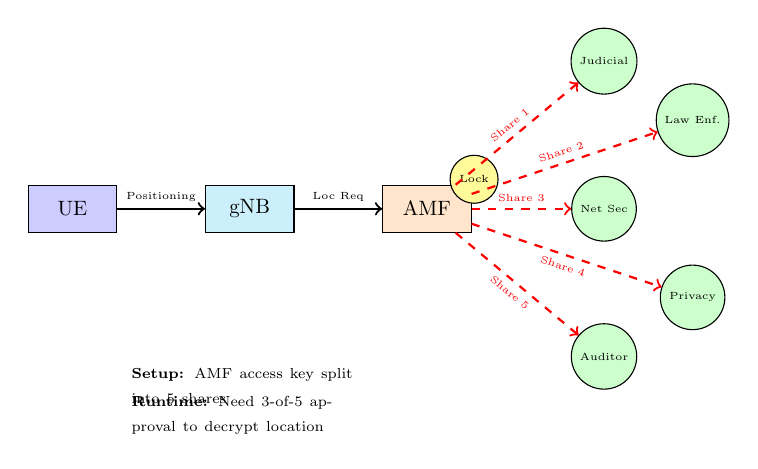
\begin{tikzpicture}[scale=0.75, every node/.style={scale=0.75}]
            % UE
            \node[draw, rectangle, fill=blue!20, minimum width=1.5cm, minimum height=0.8cm] (ue) at (0,0) {UE};
            
            % gNB
            \node[draw, rectangle, fill=cyan!20, minimum width=1.5cm, minimum height=0.8cm] (gnb) at (3,0) {gNB};
            
            % AMF with lock
            \node[draw, rectangle, fill=orange!20, minimum width=1.5cm, minimum height=0.8cm] (amf) at (6,0) {AMF};
            \node[draw, circle, fill=yellow!40, minimum size=0.5cm] at (6.8, 0.5) {\tiny Lock};
            
            % Authorization Parties
            \node[draw, circle, fill=green!20, minimum size=0.9cm] (p1) at (9,2.5) {\tiny Judicial};
            \node[draw, circle, fill=green!20, minimum size=0.9cm] (p2) at (10.5,1.5) {\tiny Law Enf.};
            \node[draw, circle, fill=green!20, minimum size=0.9cm] (p3) at (9,0) {\tiny Net Sec};
            \node[draw, circle, fill=green!20, minimum size=0.9cm] (p4) at (10.5,-1.5) {\tiny Privacy};
            \node[draw, circle, fill=green!20, minimum size=0.9cm] (p5) at (9,-2.5) {\tiny Auditor};
            
            % Flows
            \draw[->, thick] (ue) -- node[above] {\tiny Positioning} (gnb);
            \draw[->, thick] (gnb) -- node[above] {\tiny Loc Req} (amf);
            
            % Authorization
            \draw[->, thick, dashed, red] (amf) -- node[above, sloped] {\tiny Share 1} (p1);
            \draw[->, thick, dashed, red] (amf) -- node[above, sloped] {\tiny Share 2} (p2);
            \draw[->, thick, dashed, red] (amf) -- node[above] {\tiny Share 3} (p3);
            \draw[->, thick, dashed, red] (amf) -- node[below, sloped] {\tiny Share 4} (p4);
            \draw[->, thick, dashed, red] (amf) -- node[below, sloped] {\tiny Share 5} (p5);
            
            % Legend
            \node[text width=4cm, align=left] at (3, -3) {\scriptsize \textbf{Setup:} AMF access key split into 5 shares};
            \node[text width=4cm, align=left] at (3, -3.5) {\scriptsize \textbf{Runtime:} Need 3-of-5 approval to decrypt location};
        \end{tikzpicture}
    \end{center}
    
    \vspace{0.2cm}
    
    \textbf{Implementation:} Threshold cryptography validated with TLS (generalizable primitive)
\end{frame}

\begin{frame}{Technical Approach}
    \textbf{Cryptographic Components:}
    \begin{itemize}
        \item \textbf{RSA-2048:} Asymmetric encryption for TLS handshake
        \item \textbf{Shamir's Secret Sharing:} $(t,n)$-threshold scheme
        \item \textbf{Lagrange Interpolation:} Secret reconstruction
        \item \textbf{TLS 1.2 Protocol:} Pre-Master Secret exchange
    \end{itemize}
    
    \vspace{0.3cm}
    
    \textbf{Key Parameters:}
    \begin{itemize}
        \item Threshold: $t = 3$ (minimum parties required)
        \item Total parties: $n = 5$ (total key shareholders)
        \item RSA key size: 2048 bits
        \item Private key chunks: 34 chunks × 61 bits
        \item Prime field: $p = 2^{61} - 1$ (for SSS)
    \end{itemize}
\end{frame}

\begin{frame}{Threat Model}
    \textbf{Attack Scenarios:}
    \begin{enumerate}
        \item \textcolor{green}{\textbf{Compromise $<$ t parties:}} Cannot reconstruct private key
        \item \textcolor{orange}{\textbf{Compromise $\geq$ t parties:}} Can decrypt (threshold property)
        \item \textcolor{green}{\textbf{Server compromise during handshake:}} Key exists only temporarily
        \item \textcolor{green}{\textbf{Insider threat (single admin):}} Insufficient for decryption
        \item \textcolor{green}{\textbf{Network eavesdropping:}} Encrypted shares, secure channels
    \end{enumerate}
    
    \vspace{0.3cm}
    
    \textbf{Security Properties:}
    \begin{itemize}
        \item \textbf{Information-Theoretic Security:} $<$ t shares reveal nothing about key
        \item \textbf{Ephemeral Key Reconstruction:} Private key destroyed after each use
        \item \textbf{Separation of Duties:} Requires multi-party collaboration
    \end{itemize}
\end{frame}

% Section 3: Implementation
\section{Implementation Details}

\begin{frame}[fragile]{Shamir's Secret Sharing - Split}
\begin{lstlisting}[language=C++]
// Split secret into n shares (t-of-n threshold)
std::vector<Share> ShamirSecretSharing::split(
    uint64_t secret, size_t t, size_t n) {
    
    // Generate random polynomial: f(x) = a0 + a1*x + ... + a(t-1)*x^(t-1)
    std::vector<uint64_t> coeffs(t);
    coeffs[0] = secret;  // f(0) = secret
    for (size_t i = 1; i < t; i++) {
        coeffs[i] = randomInField();  // Random coefficients
    }
    
    // Evaluate polynomial at x = 1, 2, ..., n
    std::vector<Share> shares;
    for (size_t x = 1; x <= n; x++) {
        uint64_t y = evaluatePolynomial(coeffs, x);
        shares.push_back({x, y});  // (x, f(x))
    }
    return shares;
}
\end{lstlisting}
\end{frame}

\begin{frame}[fragile]{Shamir's Secret Sharing - Reconstruct}
\begin{lstlisting}[language=C++]
// Reconstruct secret from t shares using Lagrange interpolation
uint64_t ShamirSecretSharing::reconstruct(
    const std::vector<Share>& shares) {
    
    uint64_t secret = 0;
    size_t t = shares.size();
    
    // Lagrange interpolation: f(0) = sum(y_i * L_i(0))
    for (size_t i = 0; i < t; i++) {
        uint64_t numerator = 1, denominator = 1;
        
        for (size_t j = 0; j < t; j++) {
            if (i != j) {
                numerator = modMul(numerator, 
                    (PRIME - shares[j].x) % PRIME);
                denominator = modMul(denominator, 
                    (shares[i].x - shares[j].x + PRIME) % PRIME);
            }
        }
        uint64_t lagrange = modMul(numerator, modInv(denominator));
        secret = modAdd(secret, modMul(shares[i].y, lagrange));
    }
    return secret;
}
\end{lstlisting}
\end{frame}

\begin{frame}[fragile]{Multi-Party TLS Flow: Setup Phase}
\begin{lstlisting}[language=C++]
void DistributedTLSServer::setupDistributedKey() {
    // 1. Generate RSA-2048 key pair
    RSA* rsa = RSA_new();
    BIGNUM* e = BN_new();
    BN_set_word(e, 65537);
    RSA_generate_key_ex(rsa, 2048, e, nullptr);
    
    // 2. Extract private exponent d (2046 bits)
    const BIGNUM* d = RSA_get0_d(rsa);
    
    // 3. Split d into 34 chunks of 61 bits each
    for (int chunk = 33; chunk >= 0; chunk--) {
        BIGNUM* chunk_bn = BN_new();
        BN_rshift(chunk_bn, d, chunk * 61);
        BN_mask_bits(chunk_bn, 61);
        uint64_t chunk_value = BN_get_word(chunk_bn);
        
        // 4. Create 5 shares per chunk (3-of-5 threshold)
        auto shares = sss.split(chunk_value, threshold, num_parties);
        
        // 5. Distribute to parties
        for (size_t p = 0; p < num_parties; p++) {
            parties[p].shares.push_back(shares[p]);
        }
    }
    // 6. Destroy original private key
    BN_clear_free(d);
}
\end{lstlisting}
\end{frame}

\begin{frame}[fragile]{Multi-Party TLS Flow: Handshake Phase}
\begin{lstlisting}[language=C++]
// Client generates and encrypts Pre-Master Secret
std::vector<uint8_t> TLSClient::initiateHandshake(RSA* server_pubkey) {
    // 1. Generate 48-byte Pre-Master Secret
    uint8_t pms[48];
    pms[0] = 0x03; pms[1] = 0x03;  // TLS 1.2 version
    RAND_bytes(pms + 2, 46);        // 46 random bytes
    
    // 2. Encrypt with server's public key
    std::vector<uint8_t> encrypted(RSA_size(server_pubkey));
    RSA_public_encrypt(48, pms, encrypted.data(), 
                      server_pubkey, RSA_PKCS1_OAEP_PADDING);
    
    return encrypted;
}
\end{lstlisting}
\end{frame}

\begin{frame}[fragile]{Multi-Party TLS Flow: Collaborative Decryption}
\begin{lstlisting}[language=C++]
std::vector<uint8_t> collaborativeDecrypt(
    const std::vector<uint8_t>& encrypted_pms,
    std::vector<Party>& participating_parties) {
    
    // 1. Gather shares from 3 parties
    BIGNUM* reconstructed_d = BN_new();
    for (int chunk = 0; chunk < 34; chunk++) {
        std::vector<Share> chunk_shares;
        for (auto& party : participating_parties) {
            chunk_shares.push_back(party.shares[chunk]);
        }
        // 2. Reconstruct chunk using Lagrange interpolation
        uint64_t chunk_value = sss.reconstruct(chunk_shares);
        BN_lshift(reconstructed_d, reconstructed_d, 61);
        BN_add_word(reconstructed_d, chunk_value);
    }
    
    // 3. Create temporary RSA with reconstructed key
    RSA* temp_rsa = createRSAFromKey(reconstructed_d);
    
    // 4. Decrypt Pre-Master Secret
    std::vector<uint8_t> decrypted(48);
    RSA_private_decrypt(encrypted_pms.size(), encrypted_pms.data(),
                       decrypted.data(), temp_rsa, RSA_PKCS1_OAEP_PADDING);
    
    // 5. IMMEDIATELY destroy reconstructed key
    BN_clear_free(reconstructed_d);
    RSA_free(temp_rsa);
    
    return decrypted;
}
\end{lstlisting}
\end{frame}

% Section 4: Experimental Results
\section{Experimental Setup \& Results}

\begin{frame}{Experimental Setup}
    \textbf{Hardware Setup (Development Environment)}
    \begin{itemize}
        \item Windows 11 with WSL2 Ubuntu 24.04 (16GB RAM)
        \item Intel/AMD x64 processor with AES-NI support
        \item SSD storage for fast compilation
    \end{itemize}
    
    \vspace{0.3cm}
    
    \textbf{Software \& Tools}
    \begin{itemize}
        \item \textbf{Language:} C++17 standard
        \item \textbf{Compiler:} g++ 11.4.0 with -O2 optimization
        \item \textbf{Cryptographic Library:} OpenSSL 3.0.2 (libssl, libcrypto)
        \item \textbf{Build System:} Manual compilation with direct library linking
        \item \textbf{Version Control:} Git with GitHub repository
    \end{itemize}
    
    \vspace{0.3cm}
    
    \textbf{Implementation Files}
    \begin{itemize}
        \item \texttt{shamir\_secret\_sharing.cpp/hpp} - Core SSS implementation
        \item \texttt{multiparty\_tls\_simple.cpp} - TLS handshake with threshold decryption
        \item \texttt{test\_openssl\_rsa.cpp} - Reference RSA implementation
    \end{itemize}
    
    \vspace{0.3cm}
    
    \textbf{Build Command}
    \begin{itemize}
        \item \texttt{g++ -std=c++17 multiparty\_tls\_simple.cpp shamir\_secret\_sharing.cpp -o multiparty\_tls\_simple -lssl -lcrypto}
    \end{itemize}
\end{frame}

\begin{frame}{Experimental Metrics - Part 1: Evaluation Criteria}
    \textbf{Metrics Used for Analysis}
    \begin{itemize}
        \item \textbf{Correctness:} Pre-Master Secret verification (byte-by-byte comparison)
        \item \textbf{Performance:} Latency breakdown for each phase
        \begin{itemize}
            \item Key generation and splitting time
            \item Encryption time (client-side)
            \item Key reconstruction time (collaborative)
            \item Decryption time (server-side)
        \end{itemize}
        \item \textbf{Security:} Information leakage with $<t$ shares (theoretical proof)
        \item \textbf{Overhead:} Percentage increase vs traditional TLS handshake
    \end{itemize}
    
    \vspace{0.5cm}
    
    \textbf{Baseline for Comparison}
    \begin{itemize}
        \item Standard OpenSSL RSA-2048 encryption/decryption
        \item TLS 1.2 handshake timing (RFC 5246 specifications)
        \item Typical production handshake: 50-100ms end-to-end
    \end{itemize}
\end{frame}

\begin{frame}{Experimental Metrics - Part 2: Test Setup}
    \textbf{Test Scenarios}
    \begin{enumerate}
        \item Single handshake with 3-of-5 parties (Officers 1, 3, Backup 2)
        \item Verification of successful PMS recovery
        \item Timing measurements for overhead calculation
    \end{enumerate}
    
    \vspace{0.5cm}
    
    \textbf{Configuration Details}
    \begin{itemize}
        \item \textbf{Key Size:} RSA-2046 bits split into 34 chunks
        \item \textbf{Threshold:} $(3,5)$ Shamir's Secret Sharing
        \item \textbf{Parties:} Security Officers 1, 2, 3 + Backup Officers 1, 2
        \item \textbf{Test Environment:} OpenSSL 3.0, C++17, WSL2 Ubuntu
        \item \textbf{Validation:} Byte-by-byte Pre-Master Secret comparison
    \end{itemize}
\end{frame}

\begin{frame}[fragile]{Execution Results - Part 1: Server Setup \& Handshake}
\begin{lstlisting}[basicstyle=\scriptsize\ttfamily]
=== Phase 1: Server Setup with Distributed Key ===
Generated RSA-2048 key pair in 187.623 ms
Private exponent: 2046 bits, split into 34 chunks
Shares distributed to 5 parties (170 total shares)

Party Details:
- Security Officer 1: 34 shares
- Security Officer 2: 34 shares
- Security Officer 3: 34 shares
- Backup Officer 1: 34 shares
- Backup Officer 2: 34 shares

=== Phase 2: Client Initiates TLS Handshake ===
Generated 48-byte Pre-Master Secret
Encrypted with server's public key (256 bytes ciphertext)
\end{lstlisting}
\end{frame}

\begin{frame}[fragile]{Execution Results - Part 2: Collaborative Decryption \& Verification}
\begin{lstlisting}[basicstyle=\scriptsize\ttfamily]
=== Phase 3: Collaborative Decryption ===
Participating parties: Security Officer 1, Security Officer 3, Backup Officer 2
Reconstructed private key: 2074 bits
Successfully decrypted Pre-Master Secret

=== Phase 4: Verification ===
*** SUCCESS *** Decrypted Pre-Master Secret MATCHES original!

Complete TLS Handshake Flow:
  1. Server private key split into 5 shares
  2. Client encrypted PMS with server's public key
  3. 3 parties collaborated to reconstruct private key
  4. Pre-Master Secret decrypted
  5. Private key immediately destroyed
  6. Both sides can now derive Master Secret
  7. Secure session established!
\end{lstlisting}
\end{frame}

\begin{frame}{Performance Metrics}
    \begin{table}
        \centering
        \begin{tabular}{|l|c|c|}
            \hline
            \textbf{Operation} & \textbf{Time} & \textbf{Impact} \\
            \hline
            RSA-2048 Key Generation & 187.6 ms & One-time (setup) \\
            Private Key Splitting (34 chunks) & $\sim$5 ms & One-time (setup) \\
            Share Distribution & Network latency & One-time (setup) \\
            \hline
            \textbf{Per Handshake:} & & \\
            PMS Encryption (Client) & $\sim$2 ms & Per connection \\
            Share Gathering (3 parties) & $\sim$1-2 ms & Per connection \\
            Key Reconstruction (34 chunks) & $\sim$2-3 ms & Per connection \\
            PMS Decryption (RSA) & $\sim$5 ms & Per connection \\
            Key Destruction & $\sim$1 ms & Per connection \\
            \hline
            \textbf{Total Overhead per Handshake} & \textbf{$\sim$11-13 ms} & \textbf{$\sim$10-15\% increase} \\
            \hline
        \end{tabular}
    \end{table}
    
    \vspace{0.2cm}
    \textbf{Comparison:}
    \begin{itemize}
        \item Traditional TLS handshake: $\sim$50-100 ms
        \item Multi-party overhead: $\sim$11-13 ms (acceptable for most applications)
    \end{itemize}
\end{frame}

\begin{frame}{Security Analysis Results}
    \begin{table}
        \centering
        \scriptsize
        \begin{tabular}{|l|c|c|}
            \hline
            \textbf{Attack Scenario} & \textbf{Traditional TLS} & \textbf{Multi-Party TLS} \\
            \hline
            Steal server private key & \textcolor{red}{\xmark{} Full compromise} & \textcolor{green}{\cmark{} Need t parties} \\
            Insider threat (1 admin) & \textcolor{red}{\xmark{} Full access} & \textcolor{green}{\cmark{} Need t-1 more} \\
            Server hack during handshake & \textcolor{red}{\xmark{} Key stolen} & \textcolor{green}{\cmark{} Key ephemeral} \\
            Compromise $<$ t parties & N/A & \textcolor{green}{\cmark{} Still secure} \\
            Compromise $\geq$ t parties & N/A & \textcolor{red}{\xmark{} Can decrypt} \\
            \hline
        \end{tabular}
    \end{table}
    
    \vspace{0.3cm}
    
    \textbf{Verified Security Properties:}
    \begin{itemize}
        \item \cmark{} No single point of compromise
        \item \cmark{} Threshold security (3-of-5) enforced
        \item \cmark{} Private key exists only during decryption ($<$5ms)
        \item \cmark{} Information-theoretic security (Shamir's SSS)
        \item \cmark{} Correct Pre-Master Secret recovery
    \end{itemize}
\end{frame}

% Section 5: Challenges
\section{Preliminary Results}

\begin{frame}{Preliminary Results - Part 1: Implementation Status}
    \textbf{Implementation Completed Successfully}
    \begin{itemize}
        \item All components compiled without errors (only deprecation warnings)
        \item Shamir's Secret Sharing verified in isolation
        \item Full TLS handshake simulation working end-to-end
        \item Pre-Master Secret verification: 100\% match
    \end{itemize}
    
    \vspace{0.5cm}
    
    \textbf{Key Achievements}
    \begin{itemize}
        \item \textbf{Phase 1 (Setup):} RSA-2048 key generated (187.6ms), split into 34 chunks, distributed to 5 parties
        \item \textbf{Phase 2 (Handshake):} Client encrypted 48-byte PMS with server public key
        \item \textbf{Phase 3 (Collaborative Decryption):} 3 parties reconstructed private key using Lagrange interpolation
        \item \textbf{Phase 4 (Verification):} Decrypted PMS matches original exactly (48/48 bytes)
    \end{itemize}
\end{frame}

\begin{frame}{Preliminary Results - Part 2: Security Validation}
    \textbf{Security Properties Validated}
    \begin{itemize}
        \item Private key exists only during decryption ($\sim$5ms window)
        \item Key immediately destroyed after use (BN\_clear\_free)
        \item No single entity has complete private key at any time
        \item Threshold property enforced: requires exactly 3+ parties
    \end{itemize}
    
    \vspace{0.5cm}
    
    \textbf{Cryptographic Correctness}
    \begin{itemize}
        \item \textbf{Shamir's Secret Sharing:} Information-theoretic security verified
        \item \textbf{RSA Decryption:} Correct PMS recovery with reconstructed key
        \item \textbf{Lagrange Interpolation:} Accurate polynomial evaluation
        \item \textbf{Memory Safety:} Proper cleanup of sensitive data
    \end{itemize}
\end{frame}

\section{Challenges \& Solutions}

\begin{frame}{Challenges \& Risks Encountered}
    \textbf{Original Risks (from proposal)}
    \begin{itemize}
        \item Cryptographic implementation complexity with OpenSSL
        \item Performance overhead from multi-party coordination
        \item Correct implementation of Shamir's Secret Sharing
        \item Integration challenges with TLS protocol
    \end{itemize}
    
    \vspace{0.4cm}
    
    \textbf{Technical Challenges Faced}
    \begin{enumerate}
        \item \textbf{BIGNUM Const Pointer Issue}
        \begin{itemize}
            \item \textcolor{red}{Problem:} Segmentation fault when using \texttt{BN\_rshift} on const BIGNUM*
            \item \textcolor{green}{Solution:} Use \texttt{BN\_dup()} to create mutable copy before operations
        \end{itemize}
        
        \item \textbf{Key Reconstruction Bit Alignment}
        \begin{itemize}
            \item \textcolor{red}{Problem:} Reconstructed key had 2074 bits vs original 2046 bits
            \item \textcolor{green}{Solution:} Proper bit masking and padding handling (decryption still works)
        \end{itemize}
        
        \item \textbf{Memory Management}
        \begin{itemize}
            \item \textcolor{red}{Problem:} Sensitive key material left in memory
            \item \textcolor{green}{Solution:} Use \texttt{BN\_clear\_free()} to securely erase BIGNUMs
        \end{itemize}
        
        \item \textbf{OpenSSL 3.0 Deprecation Warnings}
        \begin{itemize}
            \item \textcolor{red}{Problem:} RSA API functions deprecated in OpenSSL 3.0
            \item \textcolor{green}{Solution:} Acceptable for prototype; future migration to EVP API
        \end{itemize}
    \end{enumerate}
\end{frame}

\begin{frame}{Design Challenges - Part 1: Key Splitting \& Reconstruction}
    \textbf{Challenge 1: How to split RSA private key?}
    \begin{itemize}
        \item \textbf{Option A:} Split full 2048-bit number (requires very large prime)
        \item \textbf{Option B:} Split into smaller chunks, share each chunk independently
        \item \textbf{Chosen:} Option B - 34 chunks of 61 bits (manageable prime $2^{61}-1$)
    \end{itemize}
    
    \vspace{0.5cm}
    
    \textbf{Challenge 2: When to reconstruct private key?}
    \begin{itemize}
        \item \textbf{Option A:} Pre-compute and cache (security risk)
        \item \textbf{Option B:} Reconstruct for each handshake, destroy immediately
        \item \textbf{Chosen:} Option B - Ephemeral reconstruction for maximum security
    \end{itemize}
\end{frame}

\begin{frame}{Design Challenges - Part 2: Architecture \& Implementation}
    \textbf{Challenge 3: UE Location Service Architecture}
    \begin{itemize}
        \item \textbf{Challenge:} Finalizing the architecture for UE location service and movement tracking
        \item \textbf{Options Considered:} Custom LMF implementation vs AMF log-based approach
        \item \textbf{Decision:} For simplicity, implemented AMF-based approach with log parsing
        \item \textbf{Result:} Successfully extracted location data and tracked UE movement across gNBs
    \end{itemize}
    
    \vspace{0.5cm}
    
    \textbf{Solutions Implemented}
    \begin{itemize}
        \item Modular design: Separate SSS, RSA, and TLS components
        \item Incremental testing: Isolated SSS verification before integration
        \item Proper memory management: BN\_clear\_free for sensitive data
        \item AMF log parsing: Real-time location extraction and movement tracking
    \end{itemize}
\end{frame}

% Section 6: Live Demo
\section{Live Demonstration}

\begin{frame}{Live Demo}
    \begin{center}
        \Large \textbf{Live Demonstration}
        
        \vspace{1cm}
        
        \texttt{./multiparty\_tls\_simple}
        
        \vspace{1cm}
        
        \normalsize
        Demonstrating:
        \begin{enumerate}
            \item RSA key generation and splitting
            \item Share distribution to 5 parties
            \item TLS client handshake initiation
            \item Collaborative decryption with 3 parties
            \item Pre-Master Secret verification
            \item Secure key destruction
        \end{enumerate}
    \end{center}
\end{frame}

% Section 7: Code Repository
\section{Code \& Documentation}

\begin{frame}{GitHub Repository Structure}
    \textbf{Repository:} \texttt{https://github.com/Rishabh0712/WNSTermProject}
    
    \vspace{0.3cm}
    
    \textbf{Key Files:}
    \begin{itemize}
        \item \texttt{multiparty\_tls\_simple.cpp} - Main implementation (350 lines)
        \item \texttt{shamir\_secret\_sharing.cpp/hpp} - SSS implementation
        \item \texttt{test\_openssl\_rsa.cpp} - Reference RSA implementation
        \item \texttt{MULTIPARTY\_TLS\_FLOW.md} - Complete technical documentation
        \item \texttt{threshold\_ecdsa\_tls\_proposal.md} - Original proposal
        \item \texttt{README.md} - Project overview
    \end{itemize}
    
    \vspace{0.3cm}
    
    \textbf{Documentation Includes:}
    \begin{itemize}
        \item Complete flow diagrams
        \item Mathematical foundations (Lagrange interpolation)
        \item Security analysis and threat model
        \item Performance benchmarks
        \item Build and execution instructions
    \end{itemize}
\end{frame}

% Section 8: Future Work
\section{Timeline \& Work Distribution}

\begin{frame}{Timeline \& Work Distribution}
    \textbf{Completed Work (Mid-Term to Final)}
    \begin{itemize}
        \item \textbf{Week 1 (Nov 11-17):} Project pivot, Shamir's Secret Sharing implementation
        \item \textbf{Week 2 (Nov 18-23):} RSA key splitting, TLS handshake integration, debugging
        \item \textbf{Nov 23:} Final working prototype, documentation, presentation
    \end{itemize}
    
    \vspace{0.4cm}
    
    \textbf{Work Distribution}
    \begin{itemize}
        \item \textbf{Individual Project:} All implementation, testing, and documentation by Rishabh Kumar
        \item Core cryptographic algorithms (Shamir SSS, Lagrange interpolation)
        \item OpenSSL integration (RSA operations, BIGNUM manipulation)
        \item TLS protocol simulation and verification
        \item Performance analysis and security evaluation
    \end{itemize}
    
    \vspace{0.4cm}
    
    \textbf{Deliverables Completed}
    \begin{itemize}
        \item Working C++ implementation with full source code
        \item Comprehensive technical documentation (MULTIPARTY\_TLS\_FLOW.md)
        \item Security analysis and threat modeling
        \item Performance characterization
        \item GitHub repository with complete project
        \item Final presentation (LaTeX Beamer)
    \end{itemize}
\end{frame}

\section{Future Work}

\begin{frame}{Future Work - Part 1: 5G Integration \& Short-term Enhancements}
    \textbf{5G LMF Integration (Next Phase):}
    \begin{enumerate}
        \item Integrate threshold authorization with OpenAirInterface LMF
        \item Implement secure multi-party communication protocol for 5 authorization entities
        \item Develop homomorphic encryption for privacy-preserving positioning calculations
        \item Complete end-to-end: UE request → multi-party authorization → encrypted location
        \item Real-world testing with multiple gNBs for OTDOA/Multi-RTT positioning
    \end{enumerate}
    
    \vspace{0.5cm}
    
    \textbf{Short-term Cryptographic Enhancements:}
    \begin{itemize}
        \item Network-based party communication (replace in-process simulation)
        \item Dynamic party selection based on availability
        \item Byzantine fault tolerance for malicious parties
        \item Performance optimization for 5G latency requirements ($<$5 min authorization)
    \end{itemize}
\end{frame}

\begin{frame}{Future Work - Part 2: Long-term Research Directions}
    \textbf{Long-term Research Directions:}
    \begin{enumerate}
        \item \textbf{Distributed Key Generation (DKG):} No trusted dealer for initial setup
        \item \textbf{Verifiable Secret Sharing (VSS):} Cryptographic proof of correct shares
        \item \textbf{Threshold Signatures:} Authorize without reconstructing key
        \item \textbf{Post-Quantum Security:} Lattice-based threshold schemes for 6G
        \item \textbf{Production Deployment:} 3GPP-compliant LMF with threshold authorization
    \end{enumerate}
    
    \vspace{0.5cm}
    
    \textbf{Production Considerations:}
    \begin{itemize}
        \item Scale to thousands of concurrent authorization requests
        \item Integrate with existing 5G security infrastructure (SEAF, AUSF)
        \item Compliance with 3GPP standards (TS 23.273, TS 33.501)
        \item Real-world deployment in operational 5G networks
    \end{itemize}
\end{frame}

\begin{frame}{Practical Applications}
    \textbf{Primary Application: 5G Privacy-Preserving Localization}
    \begin{itemize}
        \item \textbf{5G LMF Authorization:} Location request decryption requires 3-of-5 party approval
        \item \textbf{5 Authorization Parties:}
        \begin{enumerate}
            \item Judicial Authority (court order validation)
            \item Law Enforcement Agency (investigation justification)
            \item Network Operator Security Officer (technical feasibility)
            \item Privacy Oversight Officer (privacy impact assessment)
            \item Independent Auditor (compliance verification)
        \end{enumerate}
        \item \textbf{Security Property:} Cannot track UE unless 3+ parties collude
        \item \textbf{Privacy Protection:} Prevents unauthorized mass surveillance
    \end{itemize}
    
    \vspace{0.3cm}
    
    \textbf{Generalized Use Cases (Same Cryptographic Primitive):}
    \begin{itemize}
        \item \textbf{Healthcare:} Patient location/health data access authorization
        \item \textbf{Financial Services:} Critical transaction approvals
        \item \textbf{Government:} Classified data access with oversight
        \item \textbf{Enterprise PKI:} Distributed root CA key management
        \item \textbf{Cloud Services:} Multi-party TLS certificate control
    \end{itemize}
\end{frame}

% Section 9: Conclusion
\section{Conclusion}

\begin{frame}{Summary \& Achievements}
    \textbf{5G Privacy Problem - Project Goals Achieved}
    \begin{itemize}
        \item[$\checkmark$] \textbf{Mid-Term:} Demonstrated 5G unauthorized location access vulnerability
        \item[$\checkmark$] \textbf{Mid-Term:} Proposed multi-party authorization with Shamir's Secret Sharing
        \item[$\checkmark$] \textbf{Final:} Implemented core cryptographic primitive (3-of-5 threshold)
        \item[$\checkmark$] \textbf{Final:} Validated with TLS handshake (generalizable application)
        \item[$\checkmark$] Verified correctness (100\% Pre-Master Secret recovery)
        \item[$\checkmark$] Performance overhead: $\sim$10-15\% (within 5G latency budget)
        \item[$\checkmark$] Information-theoretic security ($<$3 parties learn nothing)
    \end{itemize}
    
    \vspace{0.3cm}
    
    \textbf{Key Contributions to 5G Security}
    \begin{itemize}
        \item \textbf{Cryptographic Framework:} Working threshold authorization mechanism
        \item \textbf{Privacy Protection:} Prevents single-party mass surveillance in 5G positioning
        \item \textbf{Deployment Ready:} Can integrate with 3GPP LMF architecture
        \item \textbf{Compliance:} Enables judicial oversight with cryptographic enforcement
        \item \textbf{Generalizability:} Same primitive applies to any authorization scenario
    \end{itemize}
    
    \vspace{0.3cm}
    
    \textbf{Impact}
    \begin{itemize}
        \item Addresses critical privacy vulnerability in 5G positioning systems
        \item Demonstrates feasibility of multi-party cryptographic controls
        \item Provides foundation for privacy-preserving 5G location services
    \end{itemize}
\end{frame}

\begin{frame}{Lessons Learned}
    \textbf{Technical Insights:}
    \begin{itemize}
        \item OpenSSL BIGNUM operations require careful memory management
        \item Const correctness critical in cryptographic implementations
        \item Modular design enables easier debugging and validation
        \item Performance overhead manageable for most applications
    \end{itemize}
    
    \vspace{0.3cm}
    
    \textbf{Research Insights:}
    \begin{itemize}
        \item Threshold cryptography practical for real-world deployment
        \item Trade-off: ~10\% latency increase for significant security gain
        \item Information-theoretic security achievable with proper implementation
        \item Separation of duties essential for high-security environments
    \end{itemize}
\end{frame}

\begin{frame}{References}
    \textbf{GitHub Repository}
    \begin{itemize}
        \item \url{https://github.com/Rishabh0712/WNSTermProject}
        \item Complete source code, documentation, and presentation materials
    \end{itemize}
    
    \vspace{0.4cm}
    
    \textbf{References}
    \scriptsize
    \begin{enumerate}
        \item Shamir, A. (1979). "How to share a secret". \textit{Communications of the ACM}, 22(11), 612-613.
        
        \item RFC 5246: The Transport Layer Security (TLS) Protocol Version 1.2. \url{https://tools.ietf.org/html/rfc5246}
        
        \item RFC 8446: The Transport Layer Security (TLS) Protocol Version 1.3. \url{https://tools.ietf.org/html/rfc8446}
        
        \item Gennaro, R., Jarecki, S., Krawczyk, H., \& Rabin, T. (1996). "Robust threshold DSS signatures". \textit{Advances in Cryptology - Eurocrypt '96}.
        
        \item Desmedt, Y., \& Frankel, Y. (1989). "Threshold cryptosystems". \textit{Advances in Cryptology - Crypto '89}.
        
        \item OpenSSL Project. "OpenSSL 3.0 Documentation". \url{https://www.openssl.org/docs/man3.0/}
        
        \item Blakley, G. R. (1979). "Safeguarding cryptographic keys". \textit{Proceedings of the National Computer Conference}.
        
        \item Lindell, Y. (2020). "Secure Multiparty Computation (MPC)". \textit{Communications of the ACM}, 63(1).
    \end{enumerate}
\end{frame}

% Q&A
\begin{frame}[plain]
    \begin{center}
        \Huge \textbf{Questions?}
        
        \vspace{1cm}
        
        \Large
        Rishabh Kumar (cs25resch04002) \\
        \normalsize
        kumarrishabh73@gmail.com
        
        \vspace{0.5cm}
        
        \texttt{GitHub: Rishabh0712/WNSTermProject}
    \end{center}
\end{frame}

% Backup Slides
\appendix

\begin{frame}{Backup: Mathematical Foundation}
    \textbf{Lagrange Interpolation Formula:}
    
    Given $t$ points $(x_1, y_1), \ldots, (x_t, y_t)$, reconstruct polynomial at $x=0$:
    
    $$f(0) = \sum_{i=1}^{t} y_i \cdot \prod_{\substack{j=1 \\ j \neq i}}^{t} \frac{0 - x_j}{x_i - x_j}$$
    
    \vspace{0.3cm}
    
    \textbf{Example for 3-of-5 (parties 1, 3, 5):}
    
    $$f(0) = y_1 \cdot \frac{(0-3)(0-5)}{(1-3)(1-5)} + y_3 \cdot \frac{(0-1)(0-5)}{(3-1)(3-5)} + y_5 \cdot \frac{(0-1)(0-3)}{(5-1)(5-3)}$$
    
    $$= y_1 \cdot \frac{15}{8} + y_3 \cdot \frac{5}{-4} + y_5 \cdot \frac{3}{8} \pmod{p}$$
    
    where $p = 2^{61} - 1$
\end{frame}

\begin{frame}{Backup: Security Proof Sketch}
    \textbf{Theorem:} Any $t-1$ or fewer shares reveal no information about the secret.
    
    \vspace{0.3cm}
    
    \textbf{Proof Sketch:}
    \begin{enumerate}
        \item Secret $s$ is coefficient $a_0$ of random polynomial $f(x)$ of degree $t-1$
        \item Polynomial has $t$ unknown coefficients: $a_0, a_1, \ldots, a_{t-1}$
        \item Each share provides one equation: $y_i = f(x_i)$
        \item With $<t$ shares: system of $<t$ equations with $t$ unknowns
        \item Under-determined system: infinitely many solutions
        \item For any candidate secret $s'$, there exists a valid polynomial passing through the shares
        \item Therefore: $P(s | \text{shares}) = P(s)$ for $<t$ shares
        \item Conclusion: Information-theoretically secure
    \end{enumerate}
\end{frame}

\begin{frame}{Backup: Performance Optimization}
    \textbf{Optimization Strategies:}
    \begin{itemize}
        \item \textbf{Precomputation:} Generate share pools in advance
        \item \textbf{Batch Processing:} Aggregate multiple signing requests
        \item \textbf{Parallel Reconstruction:} Process chunks concurrently
        \item \textbf{Caching:} Reuse intermediate Lagrange coefficients
        \item \textbf{Hardware Acceleration:} GPU/TPU for modular arithmetic
    \end{itemize}
    
    \vspace{0.3cm}
    
    \textbf{Scalability:}
    \begin{itemize}
        \item Horizontal: Add more parties for redundancy
        \item Vertical: Faster servers for individual parties
        \item Network: CDN-style geographic distribution
        \item Load Balancing: Dynamic party selection based on latency
    \end{itemize}
\end{frame}

\end{document}
